\subsection{Experiment 3: Enhancing Performance through Learning Rate and Model Complexity}

Experiment 3 was designed to test two hypotheses aimed at improving the generative model's performance. The first hypothesis assumes that setting a higher learning rate for the generator than for the discriminator at the outset could enhance performance. The second hypothesis suggests that improving the generator model's complexity could lead to better results. These hypotheses stem from the assumption that the generator task is more challenging than the discriminator task.

For this experiment, the discriminator model remained unchanged while the generator model had significantly more trainable parameters, totaling about 25 million. This was done by increasing the number of filters and the number of convolutional layers per deconvolutional block. The experiment utilized the same loss function (\ac{BCE}), dataset, optimizer, and hardware configuration as the previous iterations.

To test the hypotheses, the author derived the learning rates from the initial experiment. The generator learning rate was increased to $1 \times 10^{-3}$, while the discriminator learning rate remained at $1 \times 10^{-4}$. Training for this model stopped after 14 epochs because the results were comparable to those of the first iteration.

The total loss was $2.037$, calculated by adding the generator loss of $0.351$ and the discriminator loss of $1.686$.

Figure~\ref{fig:exp3_results} presents the loss and final spectrogram generated in this experiment.

\begin{figure}[!ht]
    \centering
    \begin{subfigure}{0.45\textwidth}
        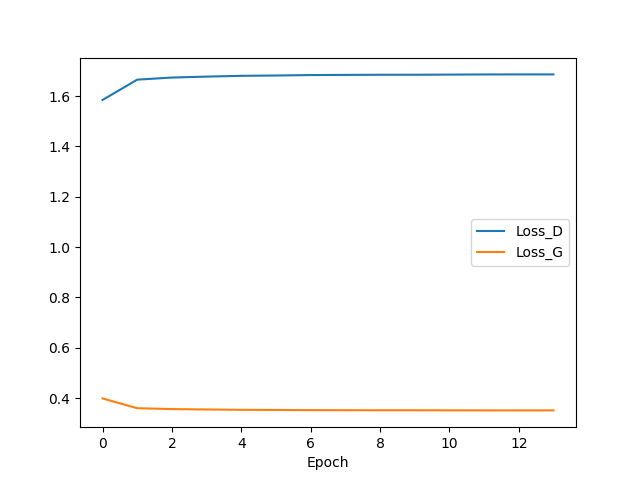
\includegraphics[width=\textwidth]{figures/4.5-results/exp3_loss.png}
        \caption{Evolving losses throughout the training process for Experiment 3.}
        \label{fig:exp3_loss}
    \end{subfigure}
    \begin{subfigure}{0.45\textwidth}
        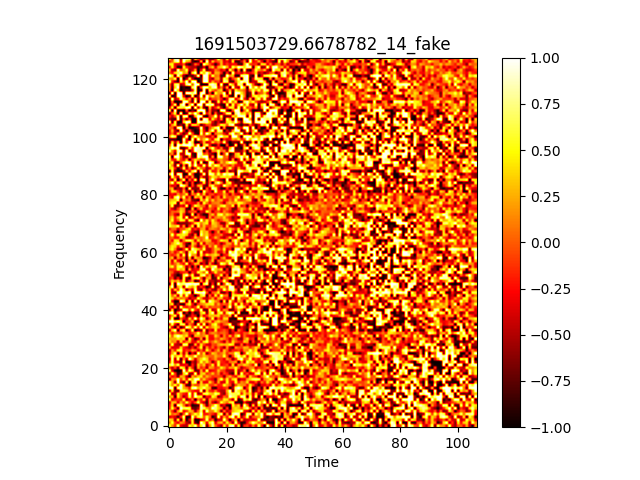
\includegraphics[width=\textwidth]{figures/4.5-results/exp3_spectrogram.png}
        \caption{Spectrogram generated in Experiment 3.}
        \label{fig:exp3_spectrogram}
    \end{subfigure}
    \caption{Results of Experiment 3.}
    \label{fig:exp3_results}
\end{figure}